\documentclass[main.tex]{subfiles}
\begin{document}
\newcommand{\Mdd}{M_\text{ДД}}
\newcommand{\Koc}{K_\text{ОС}}
\newcommand{\Ad}{A_\text{д}}
\newcommand{\ad}{\alpha_\text{д}}

\subsection{Синтез цепи обратной связи на условия заданной статической точности и необходимых
запасов устойчивости}

\subsubsection*{Определение требуемого \( K_\text{ст} \)}
По условию, синтезированная система должна обладать следующими
характеристиками качества:
\begin{itemize}
    \item запас по фазе: \( \qquad 30..60^{\circ\circ} \),
    \item запас по амплитуде: \( \qquad 8..12 \text{дБ} \)z
\end{itemize}
Статическая погрешность контролируемой величины:
\begin{itemize}
    \item \( \beta^* \leq 30'' = 1,45 \cdot 10^{-4} \) рад
    \item \( \alpha^* \leq 10'' = 4,848 \cdot 10^{-5} \) рад
\end{itemize}
Определим требуемый статический коэффициент усиления в цепи обратной связи:

 \[ K_{\text{ст.}\beta} = \frac{M_\alpha}{\beta^*} = 
    \frac{100}{1,45 \cdot 10^{-4}} = 6,897 \cdot 10^{5} \]
\[ K_{\text{ст.}\alpha} = \frac{M_\alpha}{\alpha^*} = 
\frac{100}{4,848 \cdot 10^{-5}} = 2,063 \cdot 10^{6} \]
Тогда \( K_\text{ст} = max(K_{\text{ст.}\beta}, K_{\text{ст.}\alpha}) = 2,063 \cdot 10^{6} \)

Далее рассматриваем гиросистему как объект стабилизации 
с ПФ: 
 \[ W^{\beta}_{M_{\alpha}} = \frac{-H(\Ad s^2 + \mu s + C)}{\Delta}, \]
 \[ \Delta = A\Ad B s^5 + \mu B(A+\Ad)s^4 + (\Ad H^2+BC(A+\Ad))s^3 + \] 
        \[+ H(\Ad\Koc+H\mu)s^2 + H(CH+\Koc\mu)s + CH\Koc. \] \par

ПФ разомкнутой системы выглядит следующим образом: 
 \[ W_\text{раз} = K_\text{ст.} W^{\beta}_{M_{\alpha}}|_{K_{OC}=0} \] 
 (принимаем \( K_{OC}=0 \), чтобы получить из исходной ПФ замкнутой системы ПФ разомкнутой).

Тогда получим:
\[ \Delta = A\Ad B s^5 + \mu B(A+\Ad)s^4 + (\Ad H^2+BC(A+\Ad))s^3 +  
        H^2\mu s^2 + CH^2s \]

и итоговую разомкнутую ПФ (знак "-" числителя выносится за пределы ОС, 
следовательно, не учитывается):

 \[ W_\text{раз} = \frac{2,063 \cdot 10^{6}}{s}\cdot
    \frac{10^5s^2+1,861 \cdot 10^{7}s+13,89 \cdot 10^{9}}
    {5 \cdot 10^{3}s^4 + 1,1166 \cdot 10^{6}s^3 + 1,8334 \cdot 10^{9}s^2 + 
    1,861 \cdot 10^{11}s + 1,389 \cdot 10^{14}}
 \]

 Строим ЛАФЧХ полученной функции:
 \begin{figure}[h]
     \center{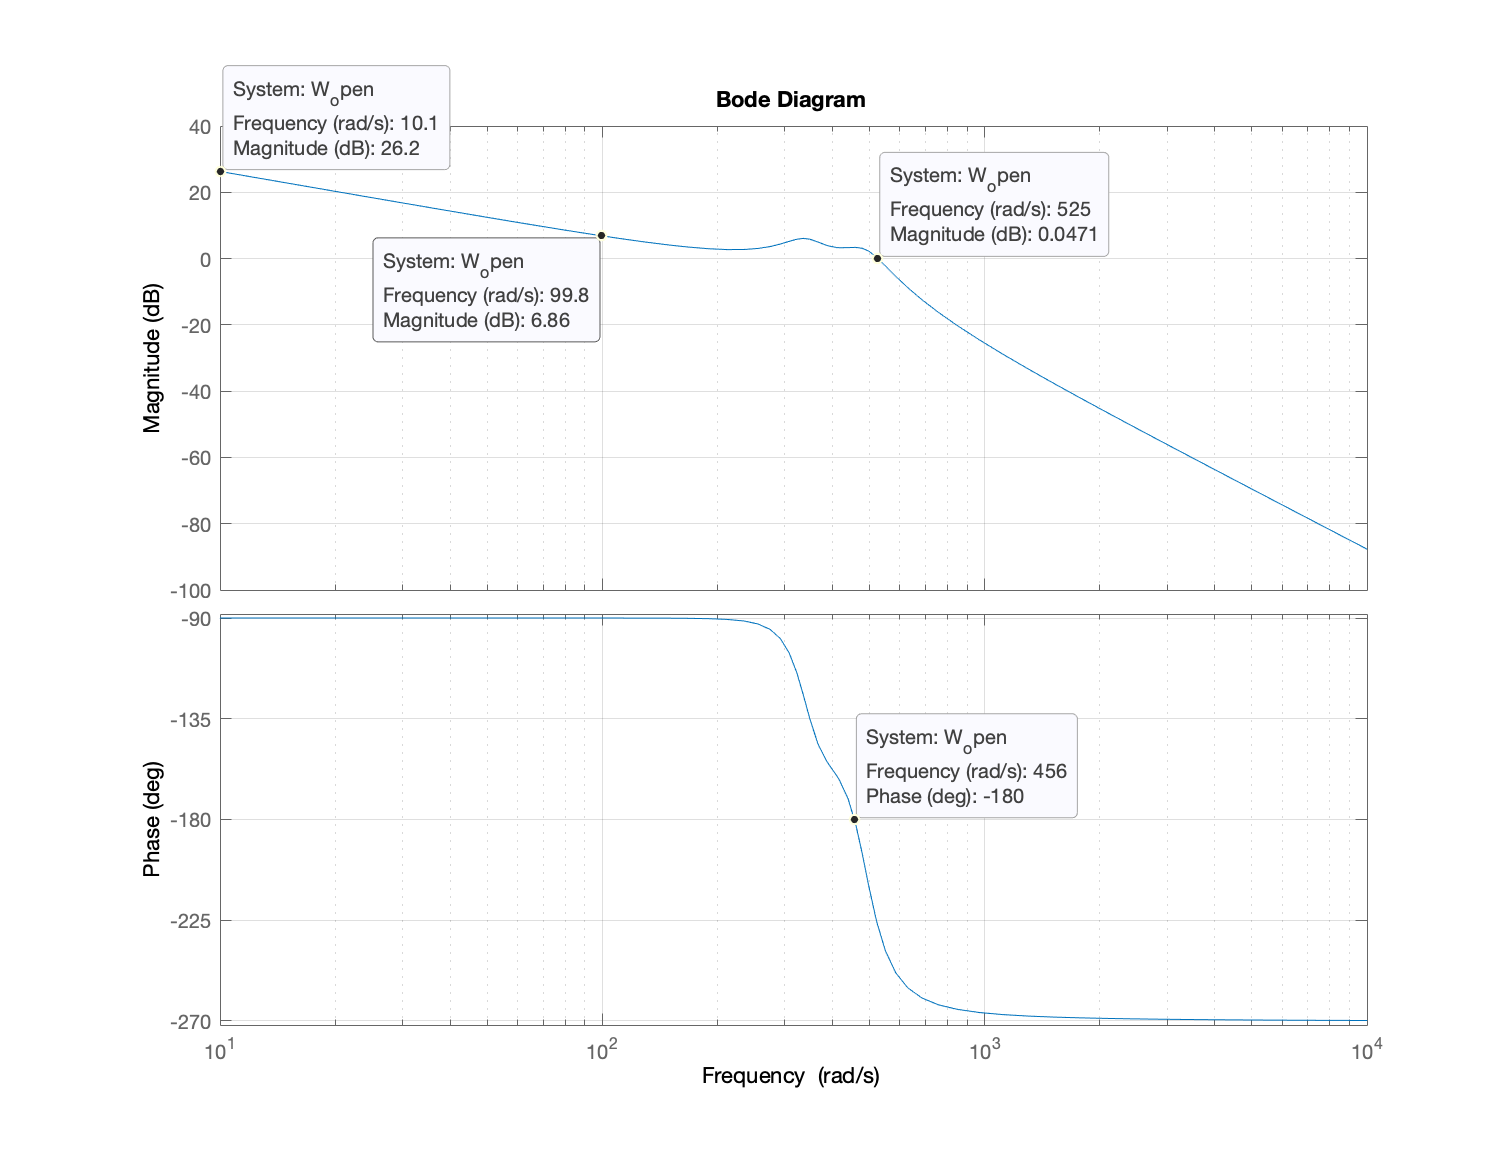
\includegraphics[width=1\linewidth]{images/p6_open_loop.png}}
     \caption{ЛФЧХ разомкнутой системы как объекта управления с заданным \( K_\text{ст.} \)}
 \end{figure}

В данном случае видно, что система неустойчива (нет запасов устойчивости, ЛФЧХ пересекает
линию -180 градусов левее частоты среза). Потому нужно синтезировать 
корректирующий контур в цепи обратной связи.

\subsubsection*{Синтез корректирующего контура в цепи ОС}
Будем пробовать скорректировать систему с помощью интегро-дифференциирующего звена
следующего вида:
 \[ W_\text{КК} = \frac{(T_2s+1)(T_4s+1)}{(T_1s+1)(T_3s+1)} \]
 По исходному ЛАФЧХ видно, что запасы устойчивости по амплидуте у системы отрицательны.
 Для приведения его в порядок нужно опустить зону "горба". Для этого введём звено
  \[ \frac{T_2s+1}{T_1s+1}, \]
при этом частота среза, очевидно уменьшится.\par 
Затем нужно обеспечить необходимый запас устойчивости по фазе, так как одним звеном,
как показали эксперименты, его не обеспечить. Для этого введём еще одно
апериодическое звено. Кроме того, чтобы сохранить исходный 
наклон характеристики на высоких частотах, для чего добавим дифференциирующее звено.
Итого добавляем следующее звено:
 \[ \frac{T_4s+1}{T_3s+1} \]

 
 Подберём численные значения коэффициентов звена. Необходимо обеспечить наклон -20 дБ 
 на частоте среза, а также необходимые значения запасов устойчивости. 
 Точку \( T_1 \) выбираем в полдекады вправо от \( \omega^0 \) = 0.316. Точку 
 \( T_2 \) подбираем так, чтобы "горб" опустился на нужную высоту,
 а частота среза оставалась левее этой точки.  Точкой \( T_3 \) дополнительно 
 корректируем запас по фазе, при этом она должна быть правее частоты среза
 с некоторым отступом (излом должен быть на амплитуде -6..12дБ). Точку 4 выберем
 там, где она не будет влиять на критическую зону, но не сильно далеко. Получили
 следующие значения:

%  Kst = 3.463e6 T1=1.5
%  \[ T_1 = 2,\quad T_2 = 0.45, \quad T_3 = 0.01, \quad T_4 = 0.002 \]

% Kst = 3.463e6
\[ T_1 = 0.316,\quad T_2 = 0.07, \quad T_3 = 0.008, \quad T_4 = 0.002 \]

 Результат представлен на рисунке ниже.
 \begin{figure}[h]
     \center{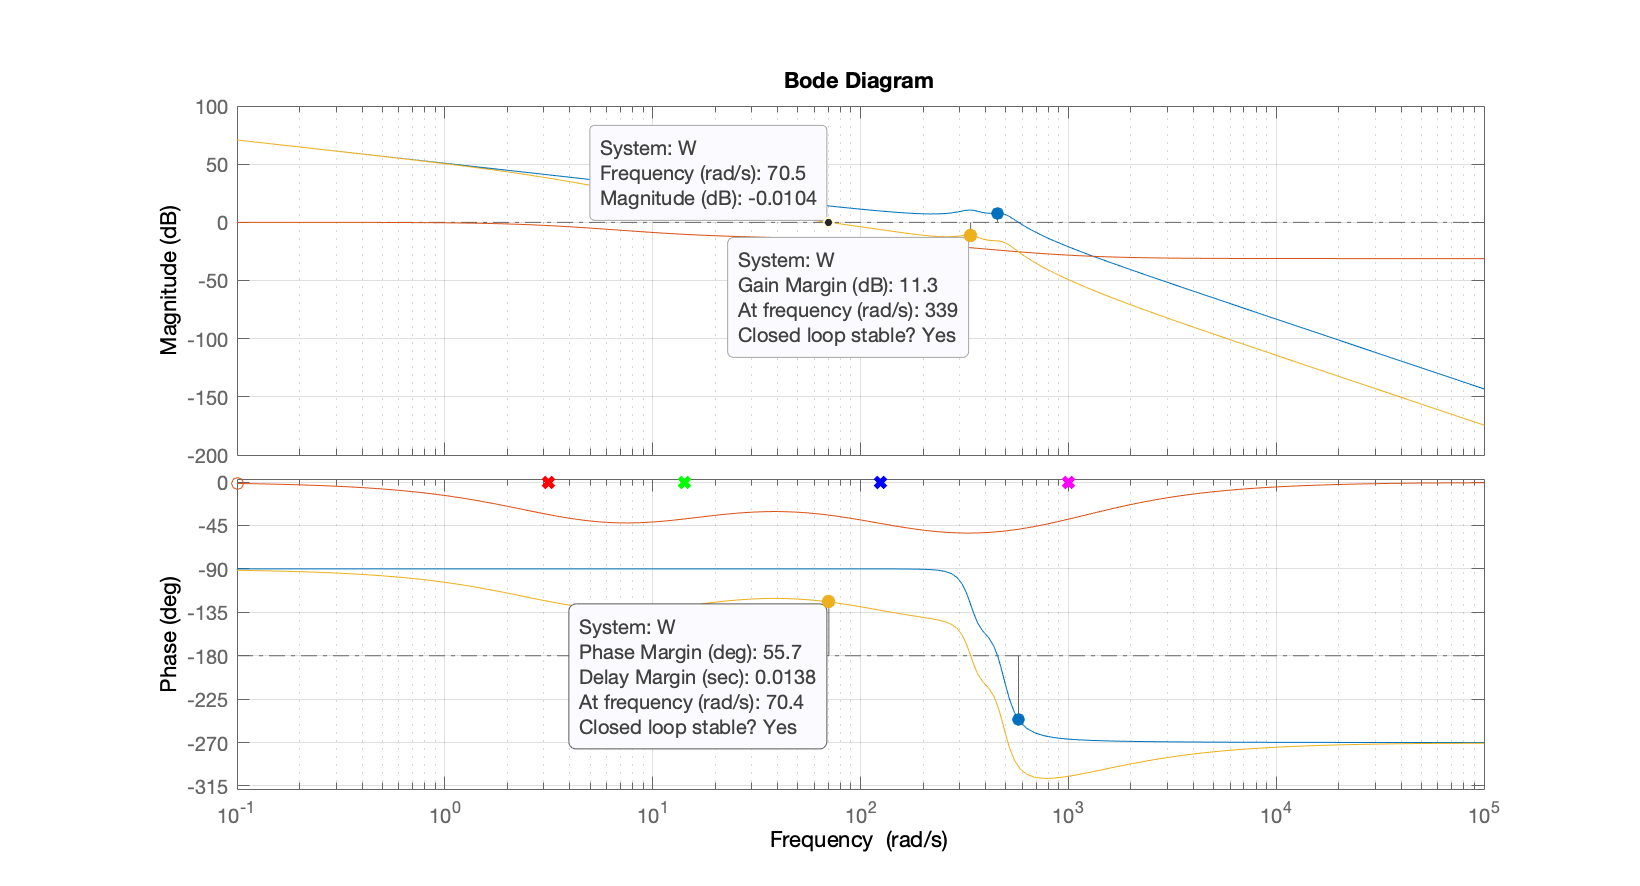
\includegraphics[width=1\linewidth]{images/p6_corrections_loop_v3.png}}
     \caption{ЛАФЧХ фильтра, разомкнутой системы без коррекции и синтезированной
     системы}
 \end{figure}

 Получили устойчивую систему со следующими запасами:
\begin{itemize}
    \item по амплитуде: \( \Delta L_m = 11.3 \text{дБ} \)
    \item по фазе: \( \Delta \varphi = 55.7^\circ \)
\end{itemize}

\subsection{Построение переходного процесса по интересующим координатам при
действии постоянного возмущающего момента}
Постоим в Simulink структурную схему замкнутой системы:
\begin{figure}[h]
    \center{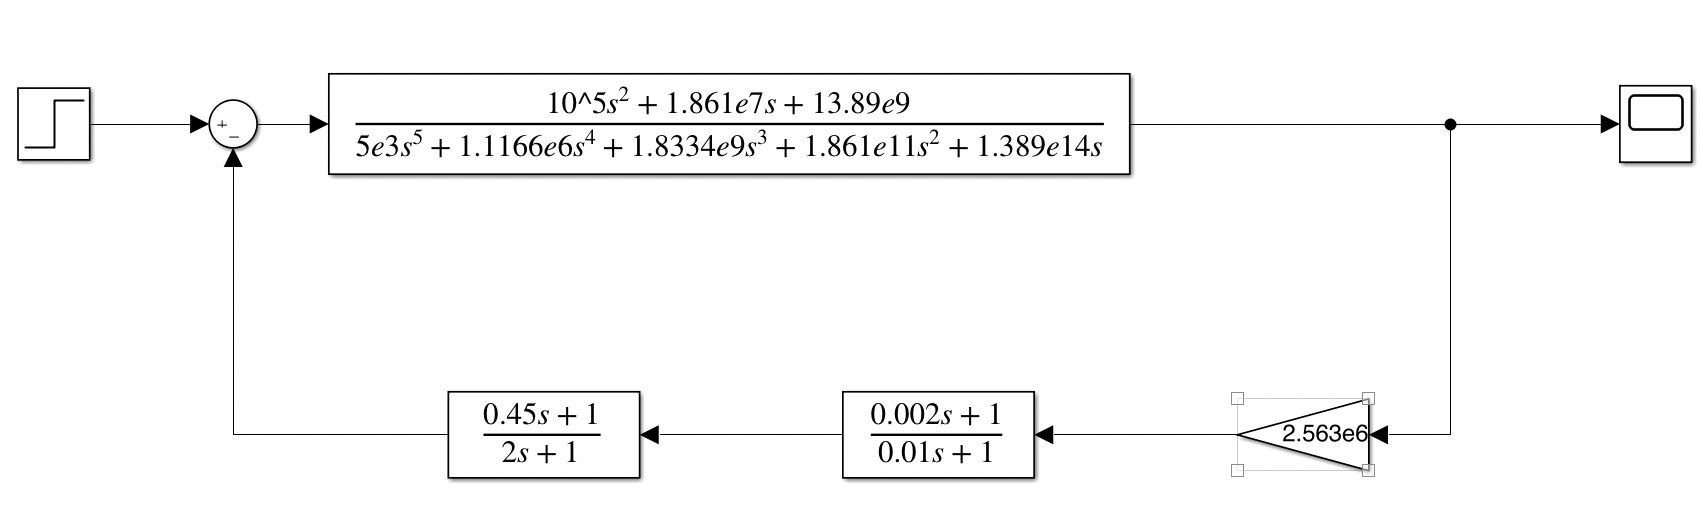
\includegraphics[width=1\linewidth]{images/p7_schema.png}}
    \caption{Структурная схема замкнутой система}
\end{figure}

Будем подавать на вход заданное по условию \( M_\alpha= \) 100гсм.
% step = 1.768; Kst=3.663e4
\begin{figure}[h]
    \center{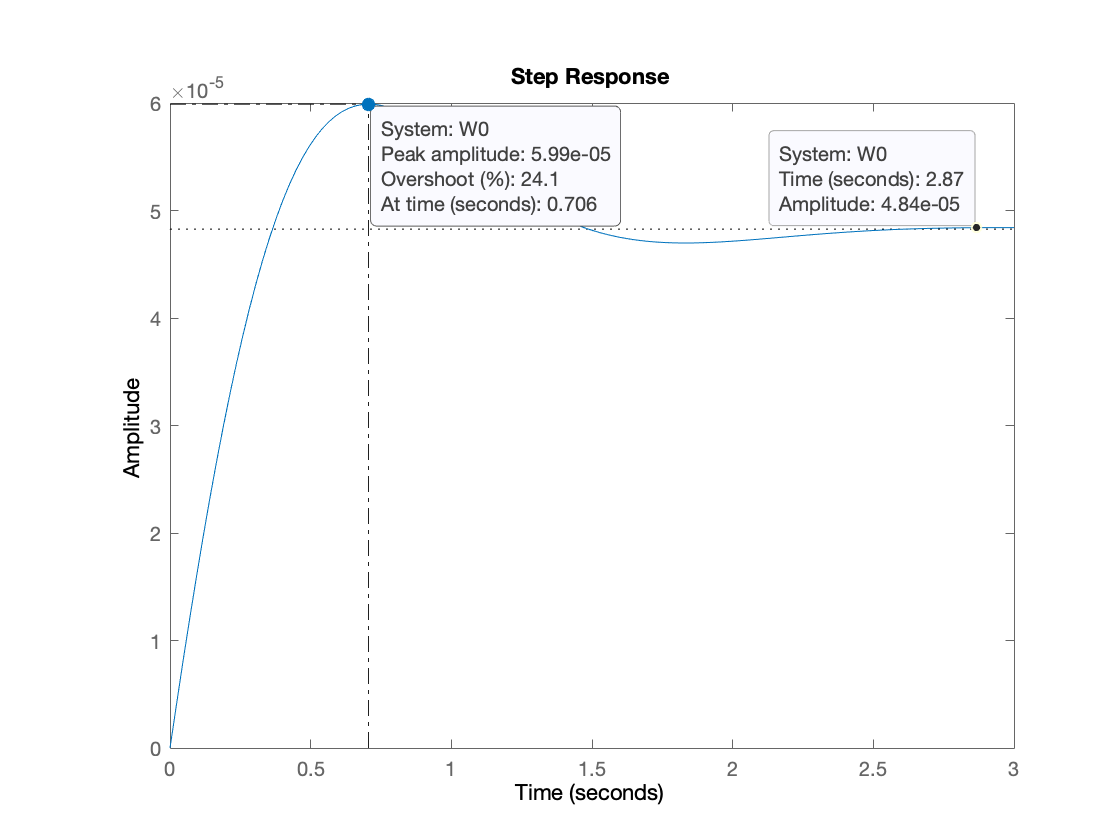
\includegraphics[width=0.7\linewidth]{images/p7_step_v3.png}}
    \caption{Переходный процесс замкнутой системы}
    \label{fig:p7_pp_corrected}
\end{figure}
На полученном графике (см. рис. \ref{fig:p7_pp_corrected}) перерегулирование равно 24.1\%, что соответствует заданным
ограничениям (не более 30\%). Усстановившееся значение \( 4.84 \cdot 10^{-5} \).

Проверим систему на выполнение требований по статической точности. Вычислим
теоретическое установившееся значение:
\[ \beta^* = \lim\limits_{s\rightarrow 0} s\cdot W_{M_\alpha}^\beta \cdot \frac{M_\alpha^*}{s} = 
 4.846 \cdot 10^{-5}\]
 Результат приблизительно равен статической погрешности по \( \beta \) и \\
 экспериментально определенному по графику.


\subsection{Построить АЧХ податливости замкнутой гиросистемы}
Передаточная функция замкнутой системы имеет следующий вид:
 \[ W_\text{замк.}(s) = \frac{W_0(s)}{1 + W_0(s)\cdot W_{reg}(s)\cdot K_{OC}(s)} \]

\[ W_\text{замк.}(s) = \frac{M(s)}{N(s)},\ \text{где} \]
    
\[ M(s) = 1500s^4 + 430150s^3 + 2.366 \cdot 10^{8}s^2 + 2.1 \cdot 10^{10} + 1.389 \cdot 10^{10}, \]

 \[ N(s) = 75s^7 + 24299s^6 + 2.92 \cdot 10^{7}s^5 + 5.75 \cdot 10^{9}s^4 + 2.49 \cdot 10^{12}s^3 + \]
 \[+ 2.53 \cdot 10^{14}s^2 + 1.313 \cdot 10^{16}s + 2.866 \cdot 10^{16} \]

\begin{figure}[h]
    \center{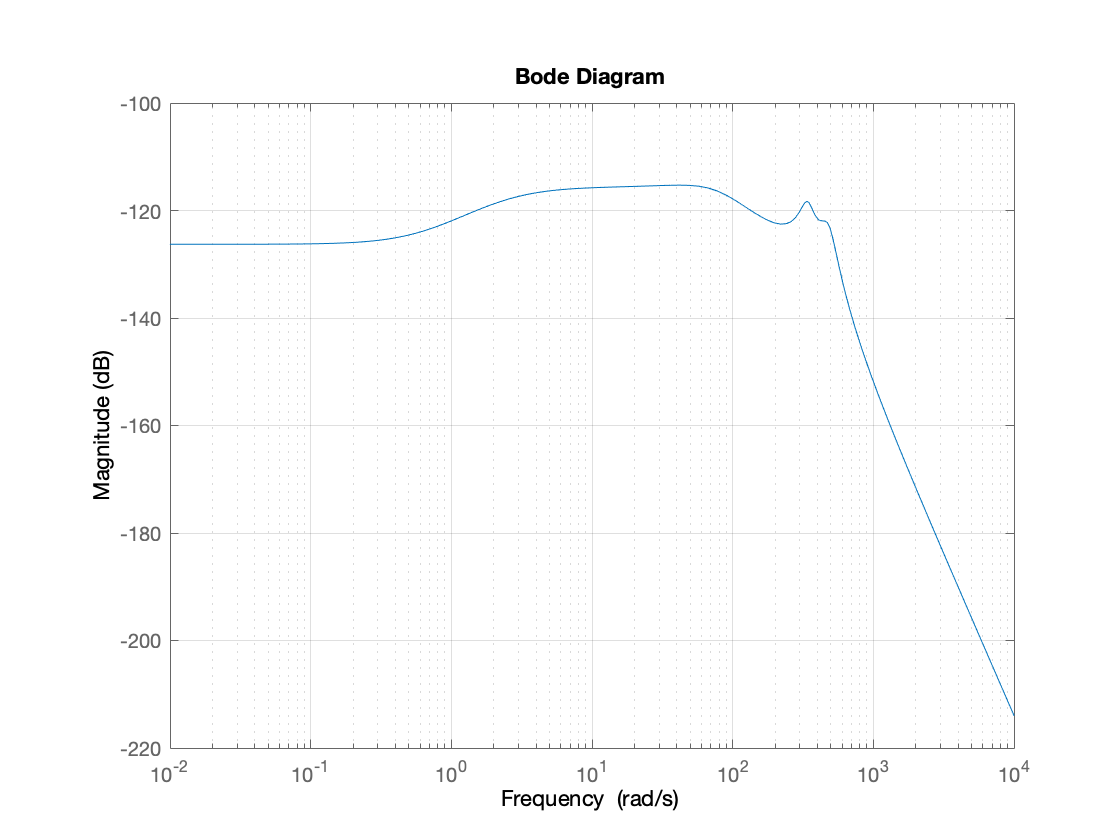
\includegraphics[width=0.8\linewidth]{images/p8_achx.png}}
    \caption{ЛАЧХ податливости замкнутой системы}
    \label{fig:p8_achx}
\end{figure}

 График представлен на рис.\ref{fig:p8_achx} 

\subsection{Построение АЧХ динамического коэффициента подавления колебаний}
Представим передаточную функцию замкнутой системы в виде:

 \[  W_\text{замк.}(s) = \frac{W_0(s)}{1 + W_0(s)\cdot W_{reg}(s)\cdot K_{OC}(s)} = \text{Ф}_*(s) \cdot W_0(s),\ \text{где} \]

\( \text{Ф}_*(s) = \frac{1}{1 + W_0(s)\cdot W_{reg}(s)\cdot K_{OC}(s)} \) - переадточная функция динамического 
коэффициента подавления колебаний.


 \[ \text{Ф}_*(s) =  \frac{M(s)}{N(s)},\ \text{где}\]
\[ M(s) = 75s^7 + 24299s^6 + 2.919 \cdot 10^{7} s^5 + 5.561 \cdot 10^{9} s^4 + 2.366 \cdot 10^{12} s^3 + \]\[+2.099 \cdot 10^{14} s^2 + 1.389 \cdot 10^{14} s \]

\[ N(s) = 75s^7 + 24299s^6 + 2.919 \cdot 10^{7} s^5 + 5.747 \cdot 10^{9} s^4 + 2.494 \cdot 10^{12} s^3 +\]\[
+ 2.533 \cdot 10^{14} s^2 + 1.313 \cdot 10^{16} s + 2.866 \cdot 10^{16} \] 
График представлен на рис. \ref{fig:p9_dyn_k}
\begin{figure}[h]
    \center{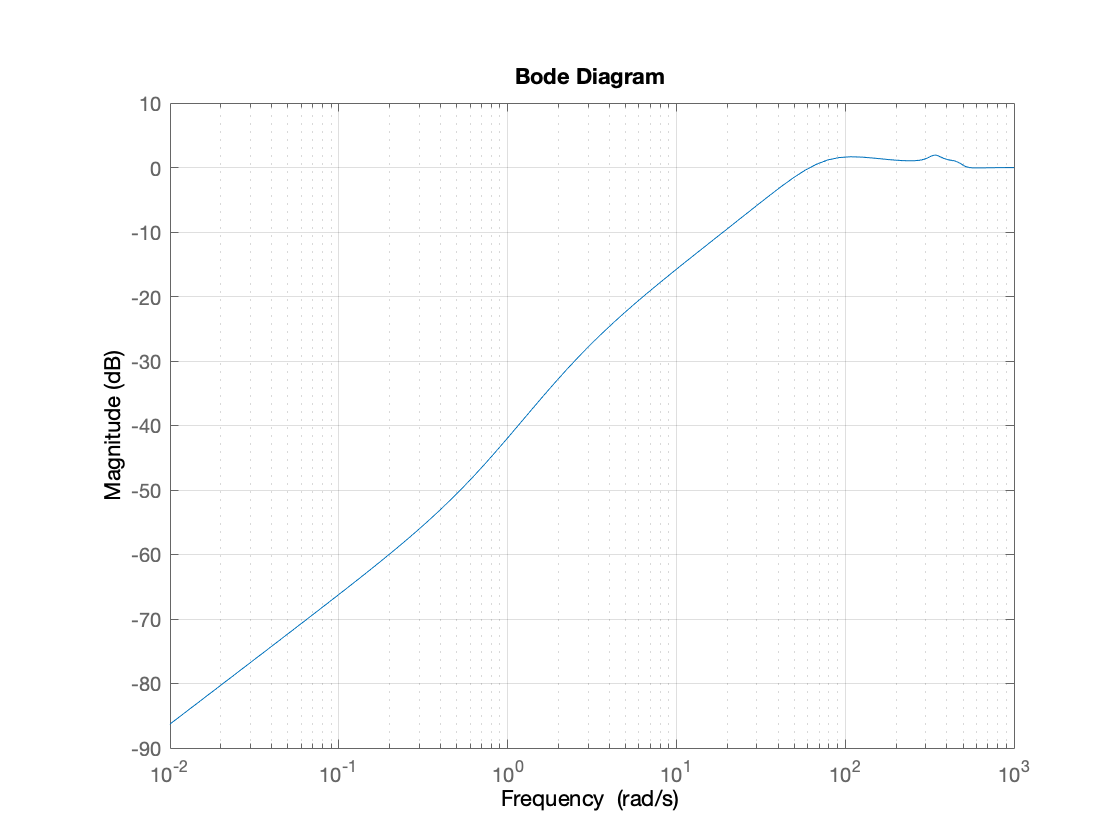
\includegraphics[width=1\linewidth]{images/p9_dyn_koef.png}}
    \caption{ЛАЧХ динамического коэффициента подавления колебаний}
    \label{fig:p9_dyn_k}
\end{figure}

\subsection{Структурная схема гиросистемы с сопутствующей нелинейностью и
преобразование ее к одноконтурной. Выражение для передаточной функции
приведенной линейной части}
По исходным уравнениям составим структурную схему с нелинейностью. Применяя структурные
преобразования, разделим в структурной схеме линейную и нелинейную составляюшие. \par 
\begin{figure}[h]
    \center{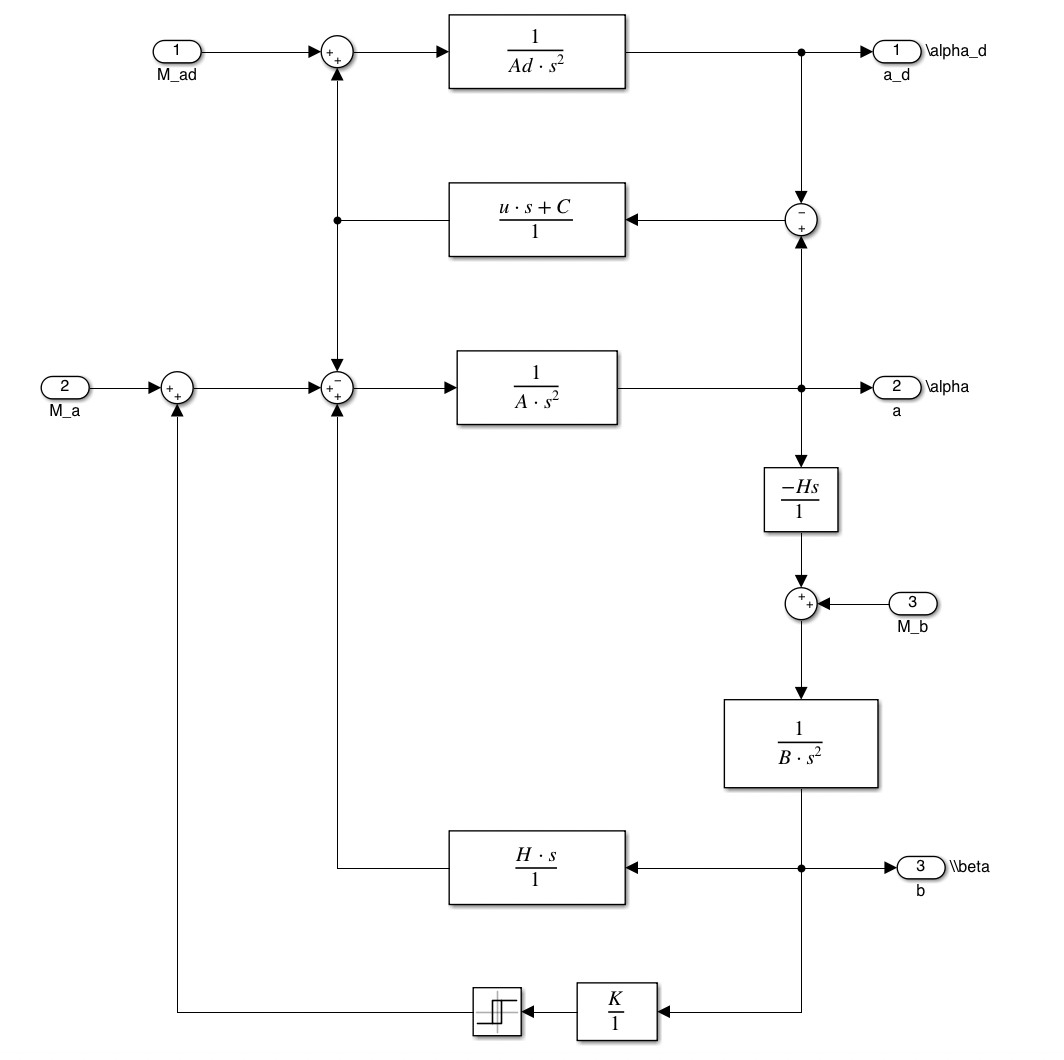
\includegraphics[width=0.8\linewidth]{images/p10_schema.png}}
    \caption{Структурная схема гиросистемы с нелинейноўстью}
\end{figure}
\begin{figure}[!h]
    \center{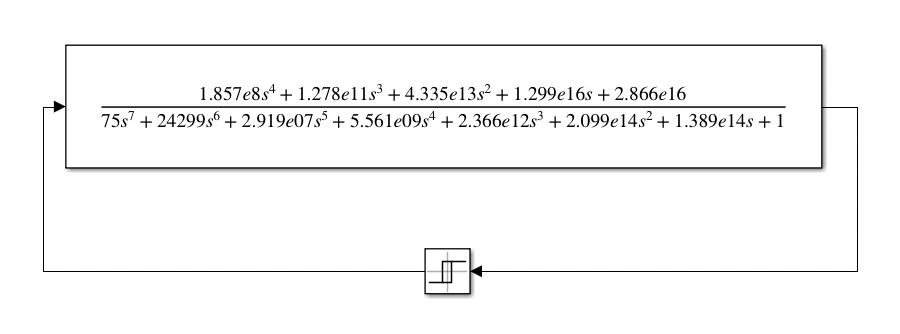
\includegraphics[width=0.8\linewidth]{images/p10_schema_2.png}}
    \caption{Структурная схема гиросистемы с разделенными линейной и нелинейной частями}
\end{figure}
Линейная часть имеет следующий вид:
 \[ W_\text{лч}(s) = K_\text{ст}\cdot W_k(s)\cdot W^\alpha_{M_\alpha}(s) \]

  \[  W_\text{лч}(s) = \frac{M(s)}{N(s)},\ \text{где}\]

\[ M(s) = 1.857e8s^4 + 1.278e11s^3 + 4.335e13s^2 + 1.299e16s + 2.866e16, \]
 \[ N(s) =   75s^7 + 24299s^6 + 2.919e07 s^5 + 5.561e09s^4 + 2.366e12s^3 +\]
 \[+ 2.099e14s^2 + 1.389e14s + 1 \]


\subsection{ Обоснование возможности применения метода гармонической линеаризации. 
Построение ЛАЧХ приведенной линейной части}

Построим ЛАЧХ приведённой линейной части (см. рис. \ref{fig:p11_lahi}) \par
\begin{figure}[!h]
    \center{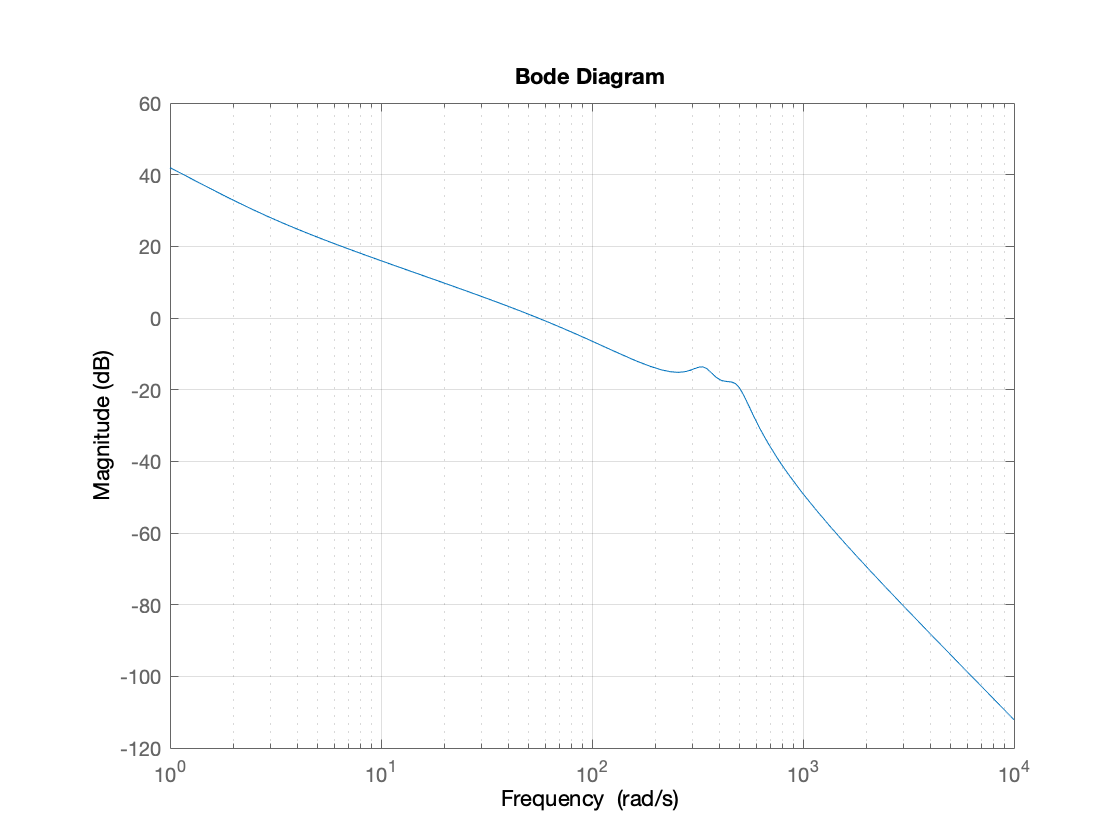
\includegraphics[width=0.8\linewidth]{images/p11_lahi.png}}
    \caption{ЛАЧХ приведённой линейной части}
    \label{fig:p11_lahi}
\end{figure}  
Как видно из ЛЧХ линейная часть системы обладает свойствами фильтра низких частот, следовательно,
 выполняется гипотеза фильтра необходимая для применения метода гармонической линеаризации.

\subsection{Гармоническая линеаризация нелинейной системы. Условие амплитудно-фазового баланса}
Сущность гармонической линеаризации заключается в замене нелинейного элемента своеобразным линейным звеном, 
коэффициент усиления которого зависит от амплитуды входного сигнала. \par
По условию задачи нелинейное звено (сухое трение в оси наружной рамки) представляет собой
 релейный 2-х позиционный элемент. При подаче на вход гармонического сигнала, 
 на выходе получим ступенчатый сигнал. Таким образом, нелинейность из входной гармоники 
 (любой ненулевой амплитуды) создаёт спектр гармоник (согласно теории Фурье) с амплитудами, 
 не зависящими от амплитуды входного сигнала. \par

\begin{figure}[h]
    \center{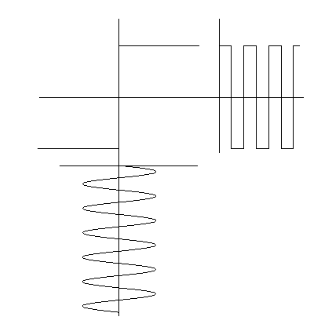
\includegraphics[width=0.5\linewidth]{images/p12_huina.png}}
    \caption{Отработка сигнала нелинейным элементом}
\end{figure}
Как мы уже установили ранее, линейная часть обладает свойством фильтра
 низких частот , она будет фильтровать все гармоники кроме первой. Таким образом, 
 на вход нелинейного элемента поступит только первая гармоника.\par 

 \subsubsection*{Проведём гармоническую линеаризацию нелинейного элемента}
\( \varphi(\dot{\alpha}) = \eta\cdot sing(\dot{\alpha}) = W_\text{нэ}\dot{\alpha}\) - сухое трение в оси наружной рамки, 
где \( \eta \) = 10 гсм - величина сухого трения. \par 

\( \alpha = A sin(\omega t) \) - входной сигнал \par 

Выход нелинейного элемента: \( \varphi(\dot{\alpha}) =
 [q(\alpha, \omega) + jq'(\alpha,\omega)]\cdot \alpha \), где

 \[ q(A,\omega) = \frac{2}{\pi\alpha}\int\limits^{2\pi}_0 \varphi(A\sin(\omega t))\sin(\omega t)d(\omega t) 
    = \frac{4\eta}{\pi A} = \frac{12.73}{A} \]
\[ q'(A,\omega) = \frac{2}{\pi\alpha}\int\limits^{2\pi}_0 \varphi(A\sin(\omega t))\cos(\omega t)d(\omega t) = 0 \]
 
Тогда ПФ нелинейного элемента:
 \[ W_\text{нэ}(A) = q(A) = \frac{12.73}{A}\]

 Периодическое (гармоническое) решение линейной системы получается при:
  \[ W_\text{лч}(j\omega)\cdot W_\text{нэ}(A) = -1 \rightarrow  W_\text{лч}(j\omega) = 
        -\frac{1}{q(A)} = -\frac{A}{12.73}\]
 
\subsection{Решение уравнения амплитудно-фазового баланса, определение параметров автоколебаний}
Инверсная характеристика линеаризованного элементы имеет вид:
 \[ f(A, \omega) = -\frac{1}{q(A)} = -\frac{\pi A}{4\eta} = -\frac{A}{12.73} \]

Построим АФЧХ приведенной линейной части и инверсную характеристику гармонически-линеаризованного 
нелинейного элемента.
\begin{figure}[h]
    \center{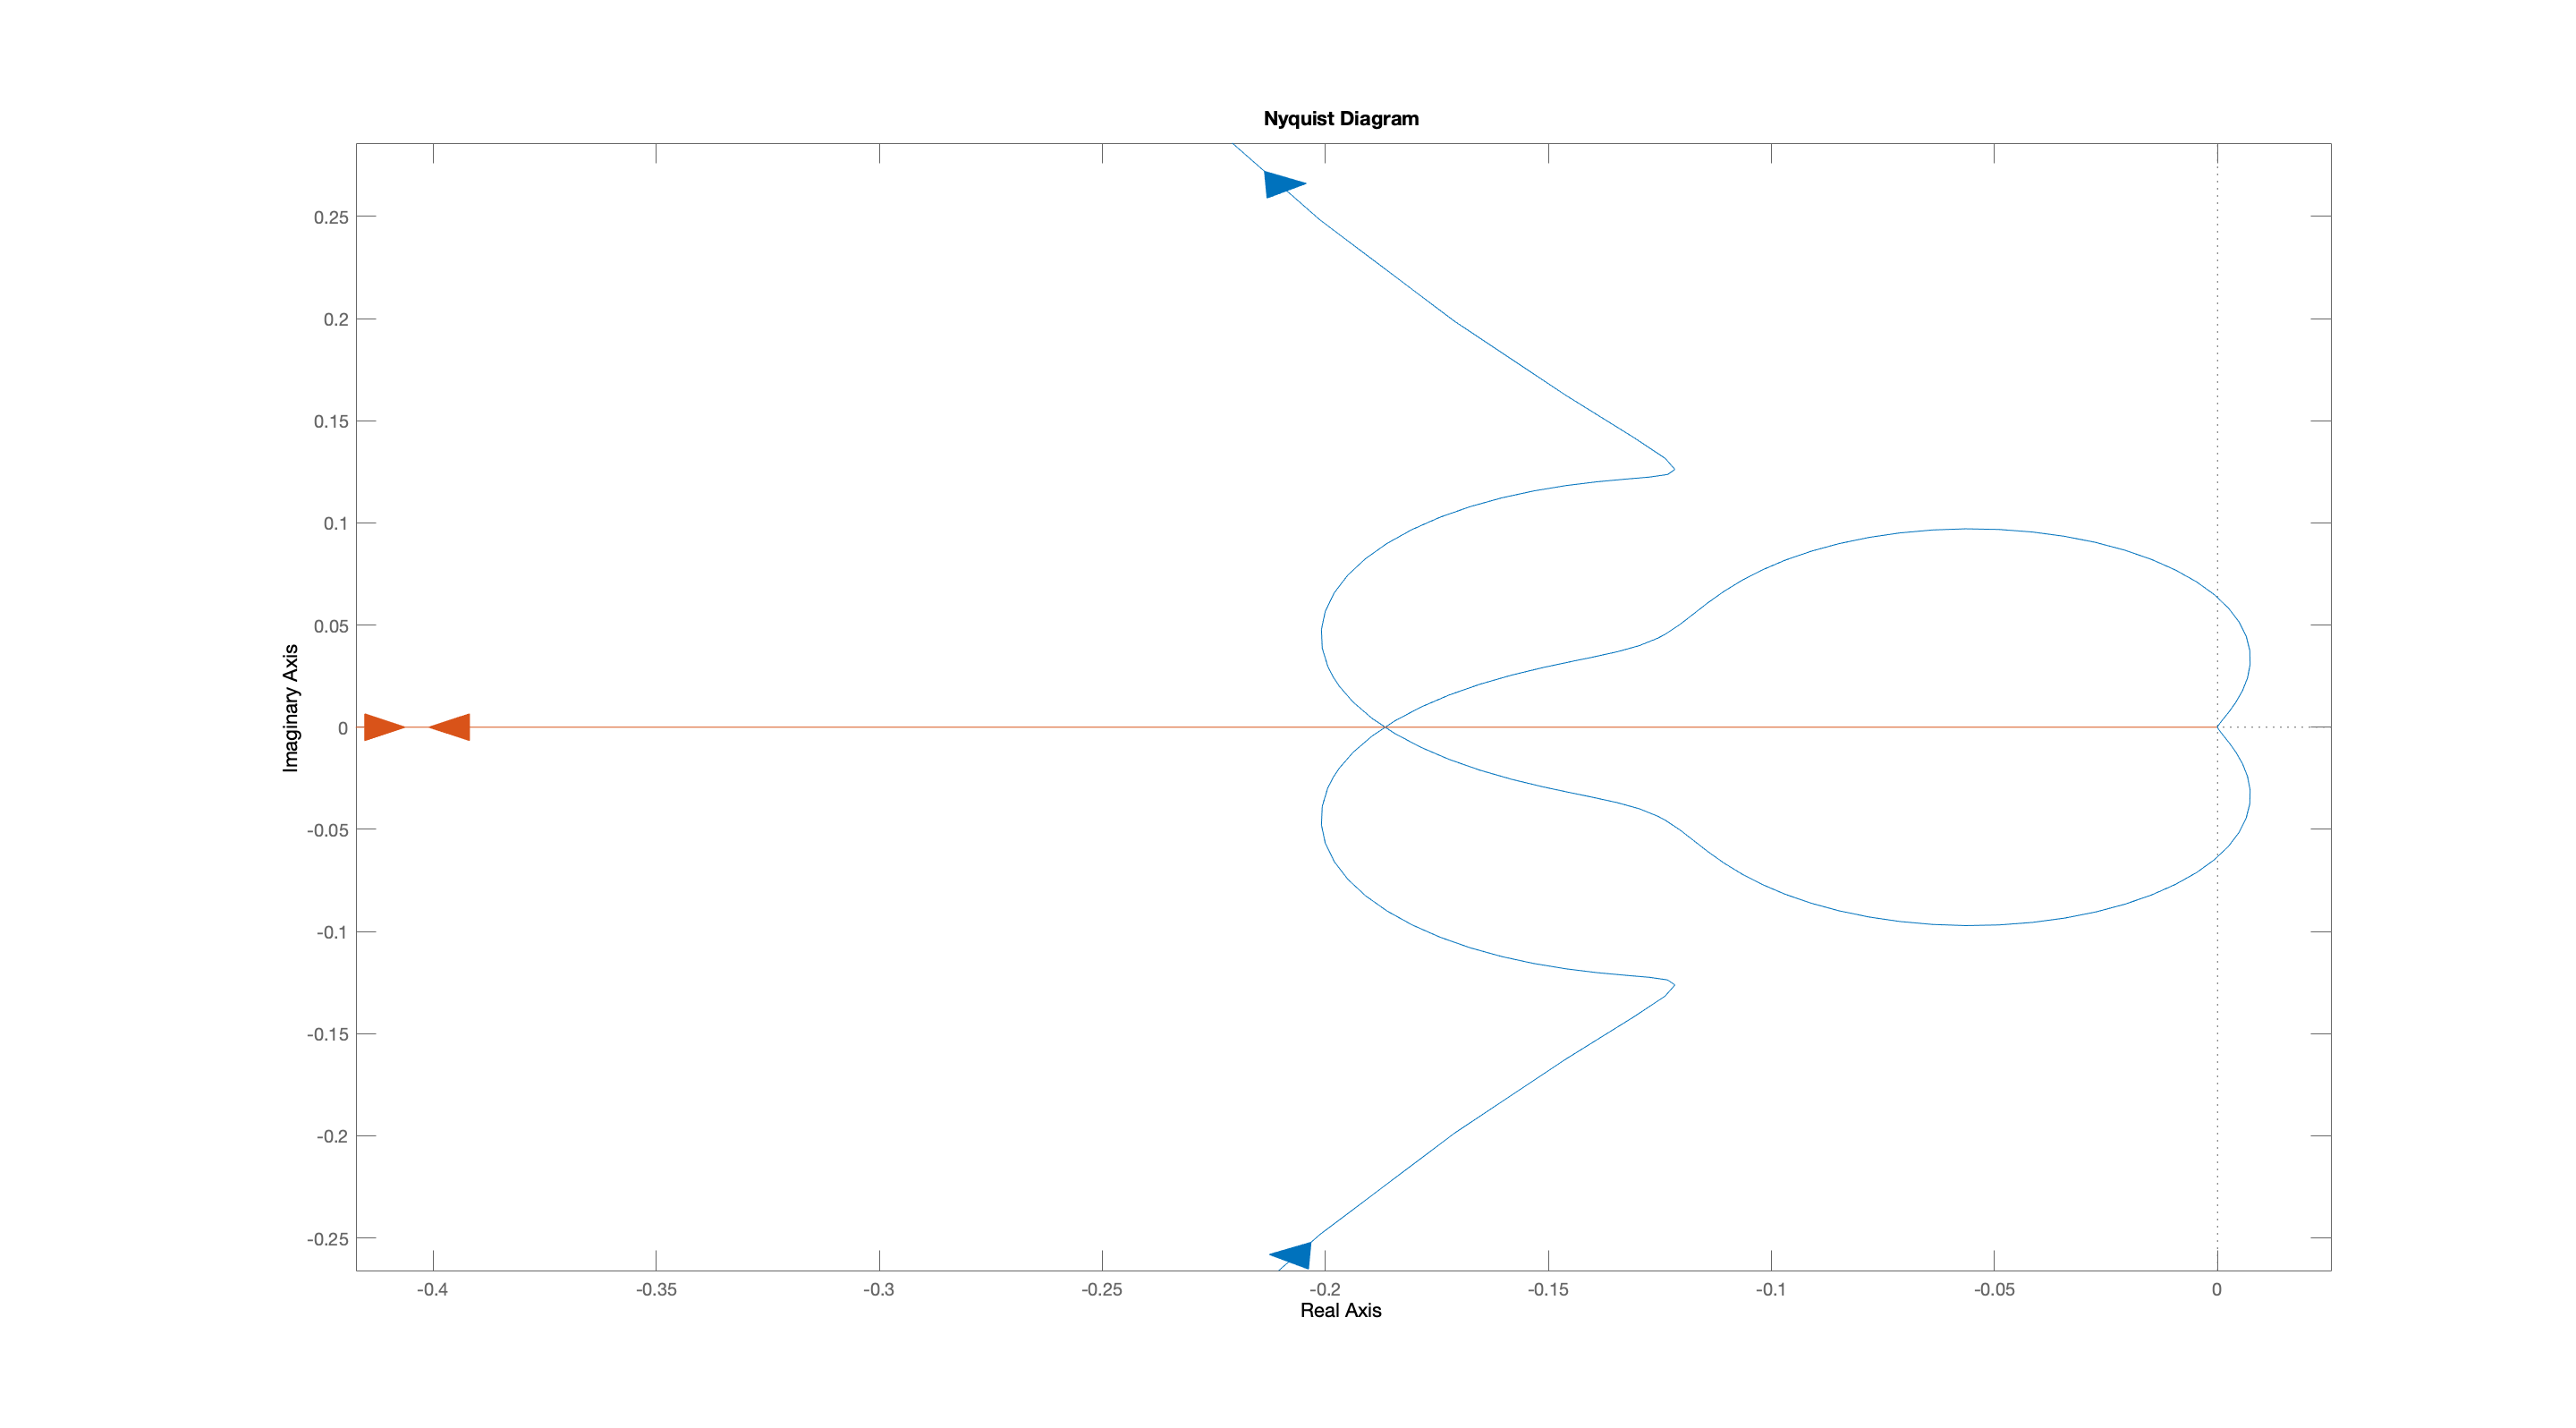
\includegraphics[width=1\linewidth]{images/p13_nyquist.png}}
    \caption{Инверсная характеристика гармонически-линеаризованного элемента и АФЧХ приведённой линейной части}
\end{figure}

В точке пересечения АФЧХ и инверсной характеристики будет выполняться условие баланса фаз, 
следовательно, возникнут автоколебания с частотой соответствующей частоте 
АФХ в этой точке \( \omega = 357 \) рад/с. Амплитуду автоколебаний определим из уравнения 
баланса фаз:
 \[ -\frac{1}{q(A)} = Re(W(j\omega)) \]
\[ -\frac{A}{12.37} = -0.187 \Rightarrow A = 1.36 \cdot 10^{-5} \]

Устойчивость автоколебаний определяется следующим образом: если при движении вдоль 
АФЧХ отрицательная действительная ось пересекается снизу - вверх, то автоколебания 
устойчивы, в противном случае – нет. В нашем случае автоколебания устойчивые с 
параметрами \( A = 1.36 \cdot 10^{-5} \) и \( \omega = 357 \) рад/с.

\subsection{Решение исходных нелинейных уравнений численными методами}

Сравним переходные процессы линейной и нелинейной системы, промоделировав их в MATLAB Simulink.

\begin{figure}[h]
    \center{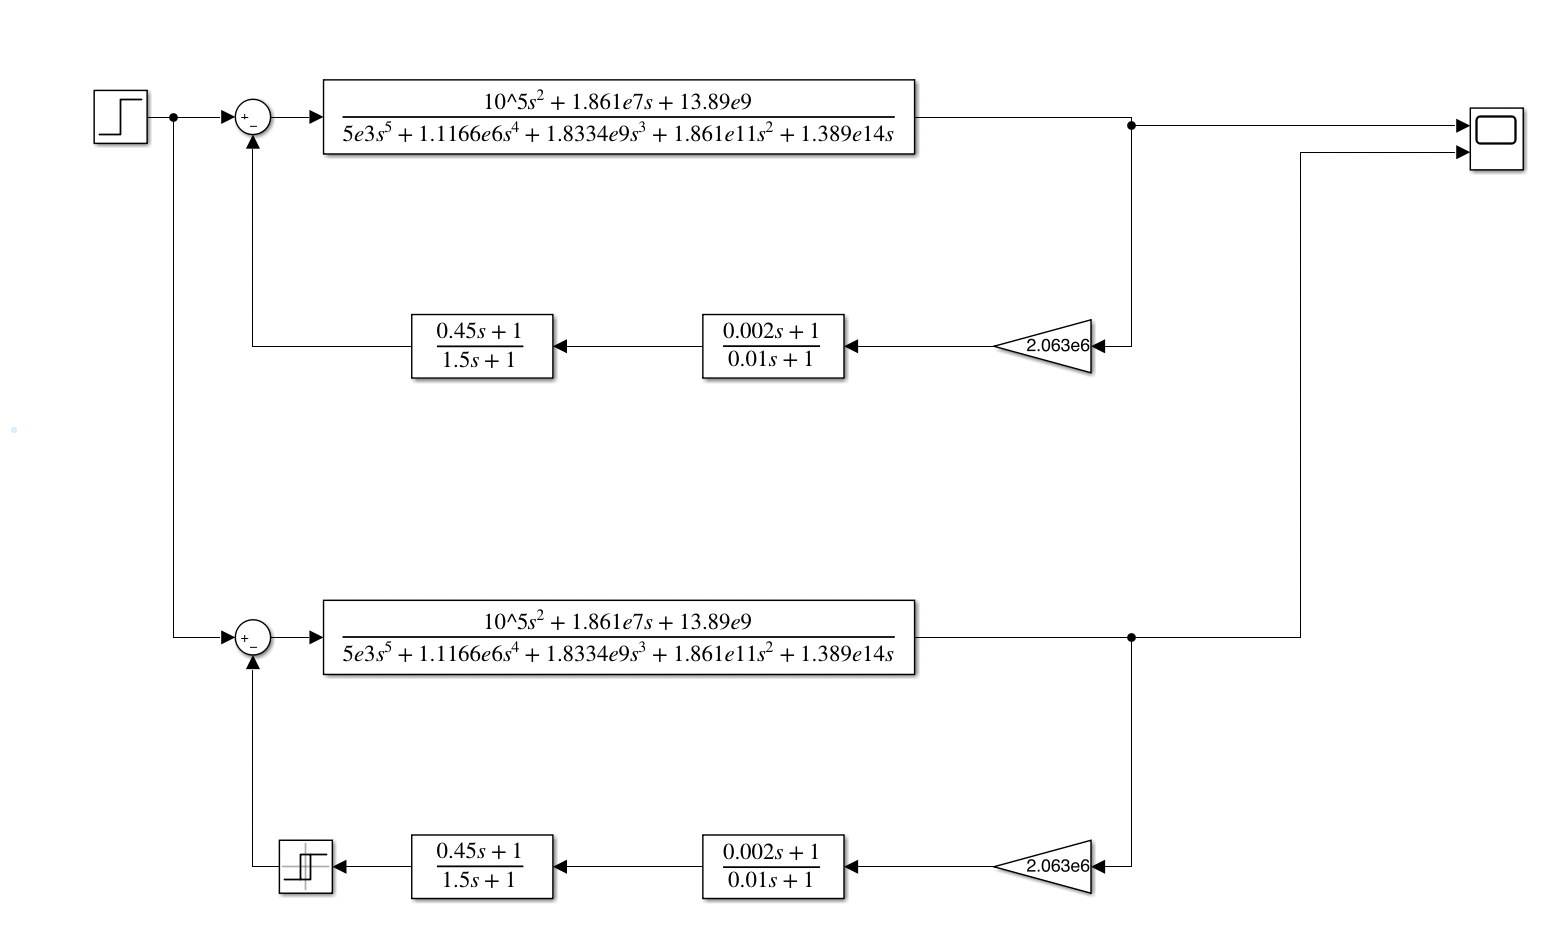
\includegraphics[width=0.8\linewidth]{images/p14_schema.png}}
    \caption{Схема для сравнения линейной и лнелинейной систем}
\end{figure}
\begin{figure}[h]
    \center{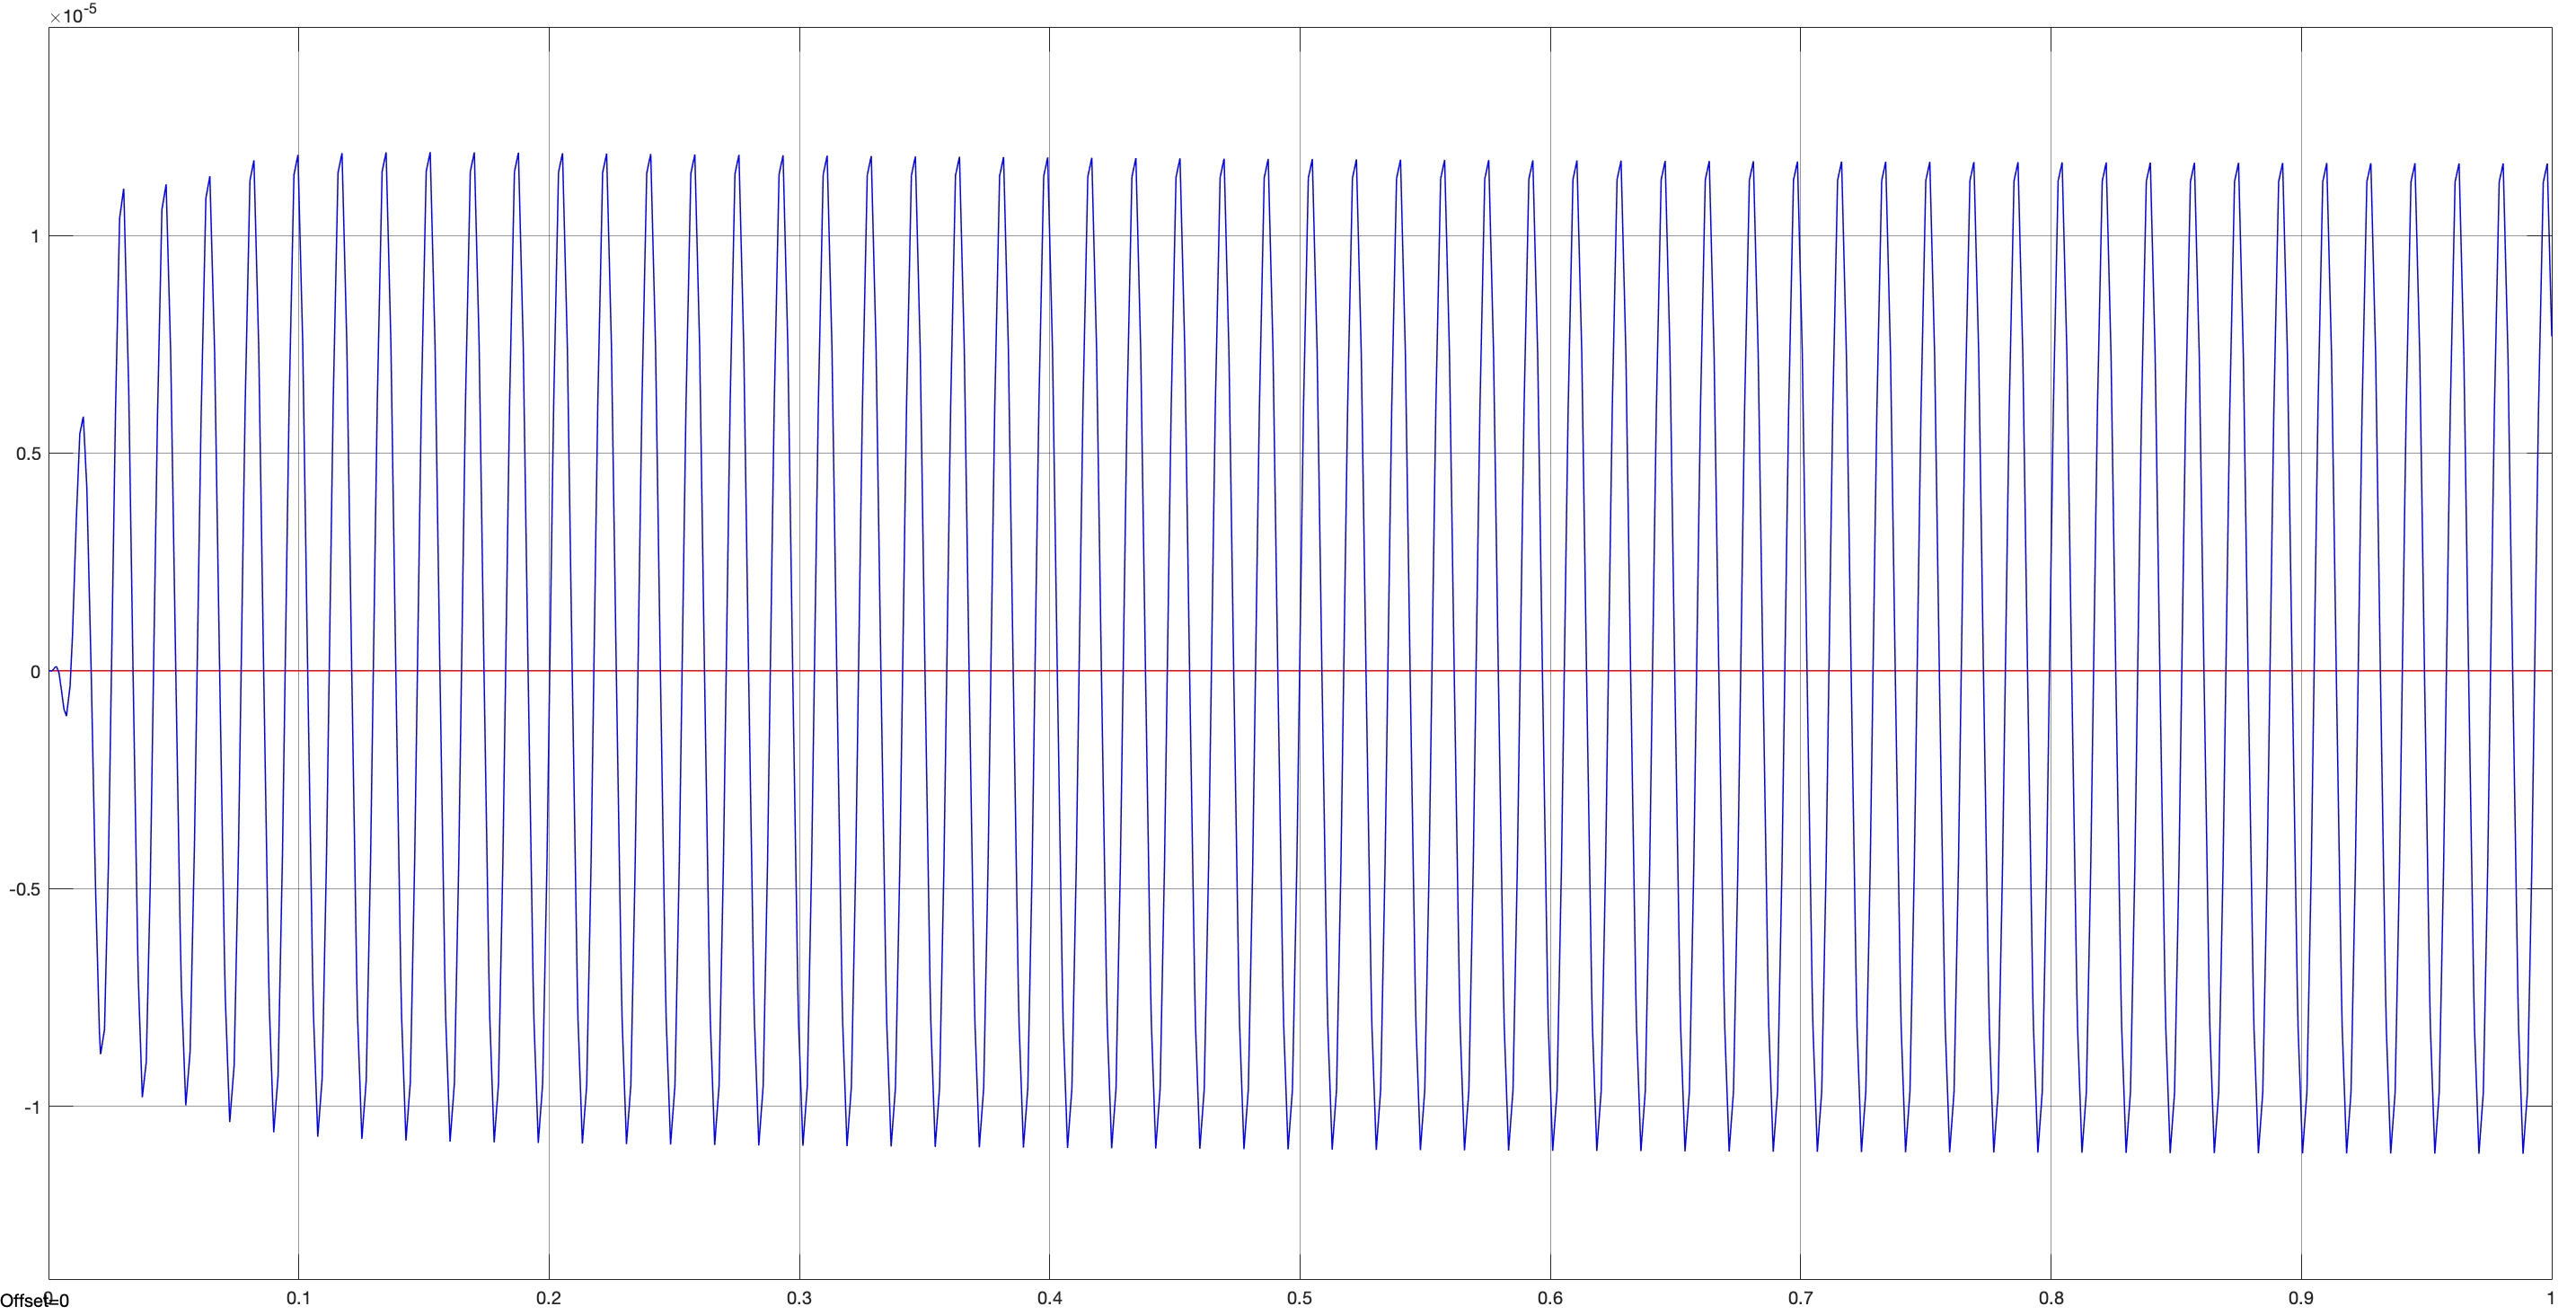
\includegraphics[width=0.8\linewidth]{images/p14_step_osc_only.png}}
    \caption{Автоколебания замкнутой системы с нелинейностью}
\end{figure}

Параметры полученного переходного процесса (\( A \approx 1.2\cdot 10^{-5},\ \omega \approx 359 \) рад/с)
довольно близки к расчётным. Различия можно списать на тот факт, что в методе гармонической 
линеаризации мы отсекаем все гармоники после первой.

\newpage
\section*{Выводы}
\addcontentsline{toc}{section}{Выводы}
В работе исследовалась гиросистема "Курсовой гироскоп" с дополнительным динамическим 
демпфером в виде сухого трения по оси наружной рамки прибора. \par 
Провели оптимизацию параметров упруго-диссипативной связи:
 \( \mu \) - коэффициента вязкого трения динамического демпфера и C -
коэффициента упругости пружин динамического демпфера. Осуществлёна коррекция путём синтеза цепи 
обратной связи на условия заданной статической точности и необходимых запасов устойчивости. Была
обоснована (т.к. ЛАЧХ приведённой линейной части обладает свойством фильтра низких
частот) и проведена гармоническая линеаризация нелинейной системы. \par

Из-за наличия в системе нелинейности могут возникать автоколебания. Это явление крайне
невыгодно, т.к. постоянная отработка автоколебаний системой приводит к быстрому износу
механических частей системы. Для исключения автоколебаний можно проводять фазовую коррекцию,
результатом которой является невыполнение условия фазового баланса, т.е. отсутствие
пересечений АФЧХ приведённой линейной части и инверсной характеристики. В данном случае для этого необходимо поставить КК который бы вносил 
отрицательный фазовый сдвиг на частотах 0,1..100 рад/с.

\newpage
\section*{Список использованных источников}
\addcontentsline{toc}{section}{Список использованных источников}
\begin{enumerate}
    \item Пельпор Д.С. «Гироскопические системы». В 3 томах. М., «Высшая школа», 1986 г.
    \item Солодовников, Плотников, Яковлев. «Теория автоматического управления
    техническими системами».
    \item Конспект лекций по курсу «Высокоточные системы навигации».
\end{enumerate}

\end{document}